\documentclass[twoside,colorback,accentcolor=tud4c,11pt]{tudreport}
%\usepackage{ngerman}

\usepackage[stable]{footmisc}
\usepackage[ngerman,pdfview=FitH,pdfstartview=FitV]{hyperref}
\usepackage{array}
\newcolumntype{L}[1]{>{\raggedright\let\newline\\\arraybackslash\hspace{0pt}}m{#1}}

\usepackage{listings}
\lstdefinestyle{BashInputStyle}{
	language=bash,
    basicstyle=\ttfamily,
	%numbers=left,
	%	numberstyle=\tiny,
	%	numbersep=3pt,
	frame=tb,
	frameshape={RYR}{Y}{Y}{RYR},
	columns=fullflexible,
	backgroundcolor=\color{gray!20},
	linewidth=0.95\linewidth,
	xleftmargin=0.1\linewidth,
  showspaces=false,
showtabs=false,
breaklines=true,
showstringspaces=false,
breakatwhitespace=true,
belowskip=1.2em,
aboveskip=1.2em,
} 

%defining a blue link:
\newcommand{\mylink}[2] {	\hyperlink{#1}{	\textit{\textcolor{blue}{#2}}}}



\usepackage{booktabs}
\usepackage{multirow}
\usepackage{longtable}

\newlength{\longtablewidth}
\setlength{\longtablewidth}{0.675\linewidth}

\title{Die fabelhaften Benner-Boys pr"asentieren
  stolz das TUD-\\Corporate-Design f"ur {\LaTeX}}
\subtitle{Clemens v. Loewenich\\Johannes Werner}
\subsubtitle{email: \textaccent{tud-design@pro-kevin.de}}
\uppertitleback{(\textaccent{\textbackslash uppertitleback})}
\lowertitleback{(\textaccent{\textbackslash lowertitleback})\hfill\today}
\institution{Speerspitze der Elite\\
    Kompetenzcenter der Leuchtt"urme\\
    Institut f"ur Angewandte Festkernphysik}
\dedication{Hier ist gen"ugend Platz\\
  f"ur eine Widmung (\textaccent{\textbackslash dedication}).\\
  \strut\\
  F"ur Annelore Schmidt\\
  aus dem Referat Kommunikation.\\
  Sie hat immer ein offenes Ohr\\
  f"ur unsere Fragen und Anregungen.}

\begin{document}
%\maketitle
 

\tableofcontents


\chapter{Item - List}
\begin{tabular}{l l l l l}
	Item & \# & Weight[g] & Weblink & Picture\\
	OpenCR Board (Controlling the motors, IMU)&1&60&\mylink{https://github.com/ROBOTIS-GIT/OpenCR/wiki/Hardware_Specification\#specification}{github\_wiki} 
	&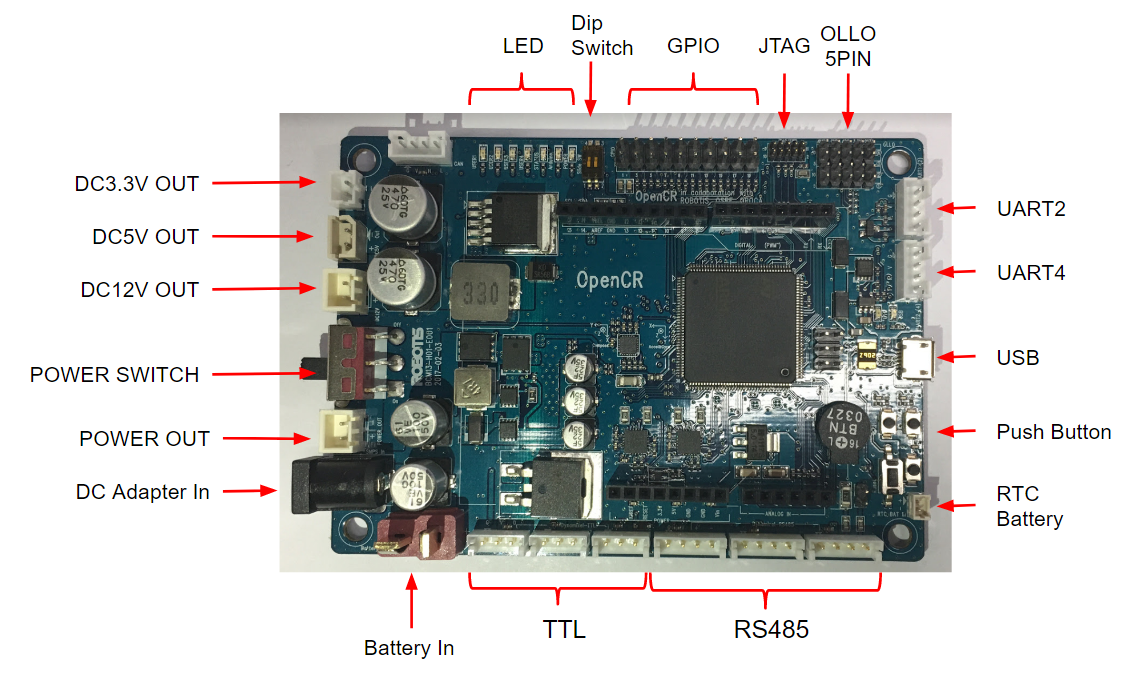
\includegraphics[width=0.1\textwidth]{img/opencr.png}  \\
	
	
	UpBoard (Main PC)&1 &80 & \mylink{arg1}{???}
	&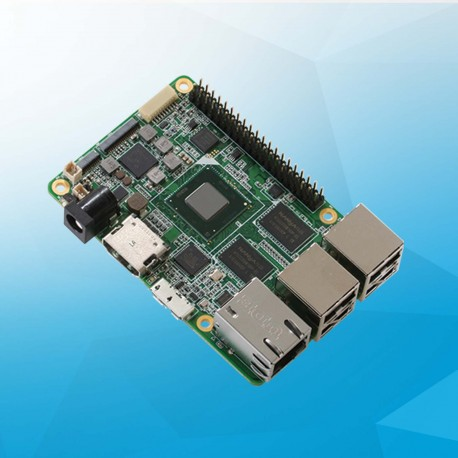
\includegraphics[width=0.1\textwidth]{img/upboard.jpg} \\
	
	Intel RealSense R200&1& 9.4& \mylink{https://www.intel.de/content/www/de/de/support/articles/000023534/emerging-technologies/intel-realsense-technology.html}{datasheet}&
	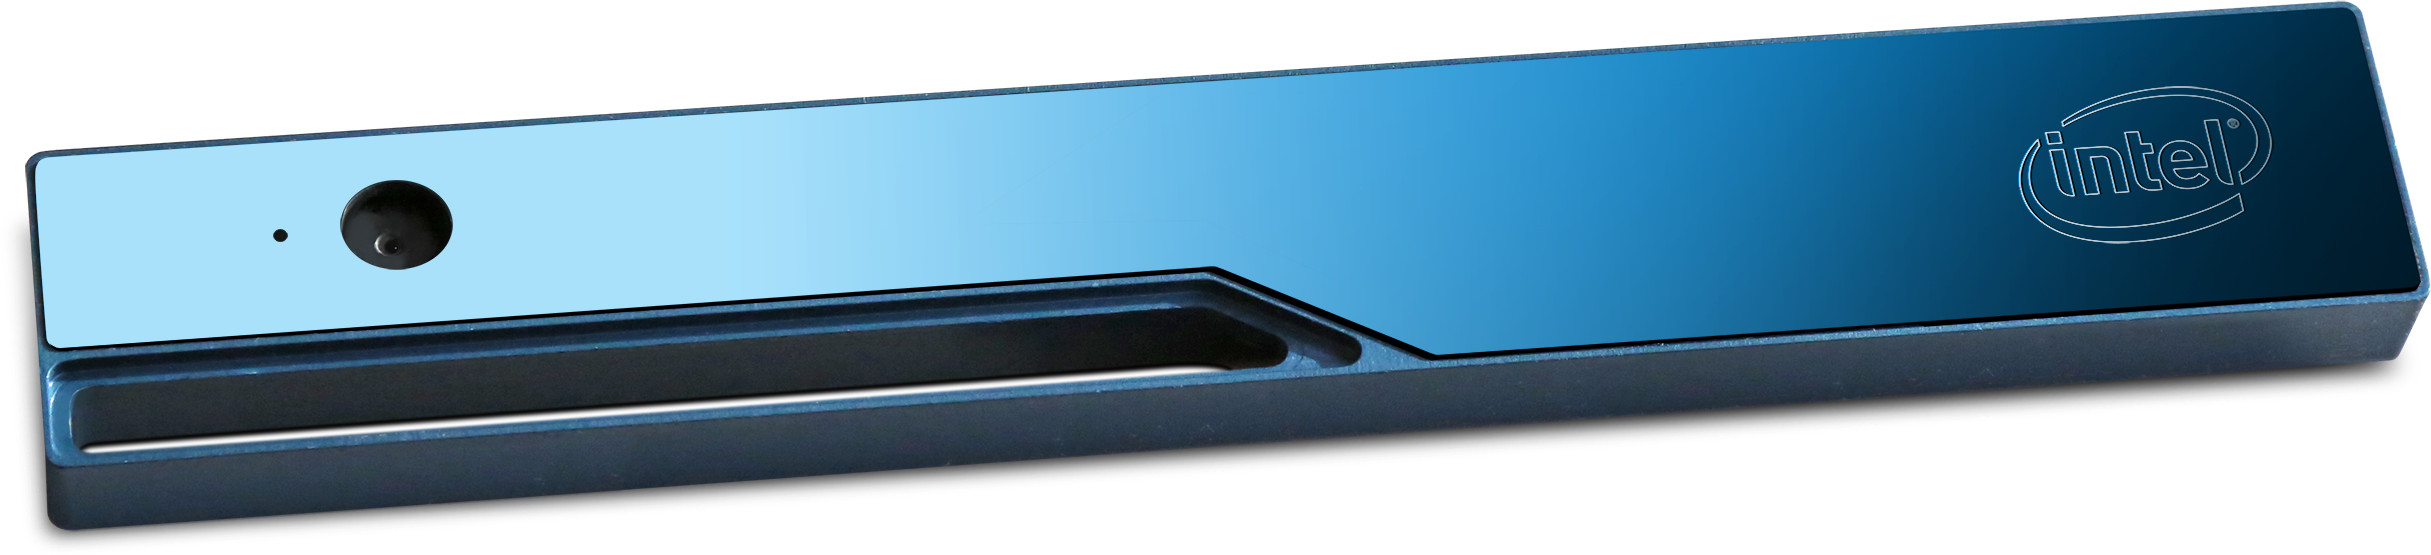
\includegraphics[width=0.1\textwidth]{img/r200.jpg} \\
	
	LaserSensor&1 & & & \\
	
	Battery: LI-PO 11.1 1800mAh LB-12 19&1& & & \\
	Turtlebot3 Layers()&4& & & \\
	XM430-W350-R Dynamixel (Motors)&3& & & \\
	
	Ball (aluminium, diameter: 140mm)&1&400 & & \\
	
	Omni wheels(dia: 60mm, thickness:25mm)&3&46 &\mylink{http://krause-robotics.de/xtshop/Antriebe/Raeder/Allseitenraeder/Allseitenraeder-60-mm:::99_100_106_114.html}{buy here} &  	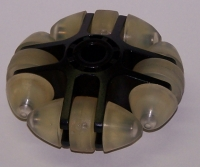
\includegraphics[width=0.1\textwidth]{img/wheel.jpg}   \\
	

	
\end{tabular}


TODO:\\
\begin{enumerate}
	\item Abmessungen von einer struckture layer
	\item welches upboard verwenden wir 2 oder das normale
\end{enumerate}

\chapter{Simulation}

\section{Launch}
These files are executed one after another:
\begin{enumerate}
	\item bb\_simulation: ballbot.launch
	\item bb\_description: bb\_description.launch
	\item bb\_description -> urdf: bb.xacro
	\item bb\_description -> urdf: bb.urdf.xacro
	\item bb\_description -> urdf: common\_properties.xacro
	\item bb\_description -> urdf: bb.gazebo.xacro
\end{enumerate}

\section{Simulation design}

Ballbot SDF Reference:
\mylink{https://bitbucket.org/osrf/gazebo/issues/2335/how-to-set-the-friction-of-ballbot-the}{Ballbotmodel} 

We use not the sdf but the xacro description as in this example \mylink{http://gazebosim.org/tutorials/?tut=ros_urdf}{here}.

\begin{center}
		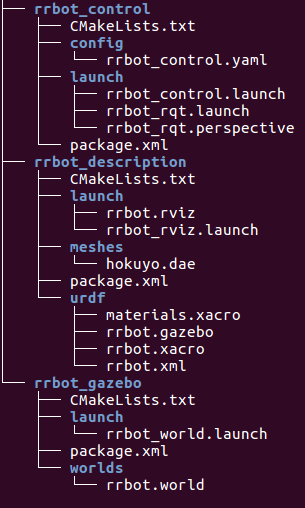
\includegraphics[width=0.2\textwidth]{img/filestructure.png} 
\end{center}

Gazebo uses different physics engines:\\
\begin{itemize}
	\item Open Dynamics Engine (ODE) (Default)
	\item Bullet
	\item Dynamic Animation and Robotics Toolkit (DART)
	\item Simbody
\end{itemize}
 which all have different friction etc. models.

Files:
\begin{itemize}
	\item bb.urdf.xacro: Link's: Visual description of the Robot and its collision model(STL file). Pose Mass and Inertias. Joint's: Pose,axis,effort and velocity limits, friction.
	\item common\_properties.xacro: Macros for color definition.
	\item bb.gazebo.xacro: gazebo references dynamics of the links: friction parameters (mu1,mu2), 
\end{itemize}

Gazebo Parameter's List:\\
\begin{tabular}{l L{12cm} l l}
	name(xacro)&description&value&sdf group\\
	mu1&is the Coulomb friction coefficient for the first friction direction&1.0&ode\\
	mu2& is the friction coefficient for the second friction direction (perpendicular to the first friction direction)&2.0&ode\\
	kp&spring constant equivalents of a contact as a function of SurfaceParams::cfm and SurfaceParams::erp & &ode \\
	kd&spring damping constant equivalents of a contact as a function of SurfaceParams::cfm and SurfaceParams::erp.   & &ode \\
	cfm&Constraint Force Mixing parameter.& &ode \\
	erp&Error Reduction Parameter.& &ode \\
	min\_depth&Minimum depth before ERP takes effect.   & &ode \\
	max\_Vel& Maximum interpenetration error correction velocity.
	If set to 0, two objects interpenetrating each other will not be pushed apart.  & &ode \\
	slip1&Artificial contact slip in the primary friction direction  & &ode \\
	slip2&Artificial contact slip in the secondary friction dirction.& &ode \\
\end{tabular}

See: \mylink{http://osrf-distributions.s3.amazonaws.com/gazebo/api/dev/classgazebo_1_1physics_1_1ODESurfaceParams.html}{ODESurfaceParams}

\section{Gazebo Parameters}

	\begin{lstlisting}[style=BashInputStyle]
git@git.sim.informatik.tu-darmstadt.de:TurtleBot/jsonlab.git
git@git.sim.informatik.tu-darmstadt.de:TurtleBot/octave_rosbridge.git
	\end{lstlisting}
	
	\section{Control}
	sobald diff drive plugin angeschaltet drehen sich die raeder viel zu schnell ....
	
	
	\subsection{Plugins}
	\begin{itemize}
		\item gazebo-ros-control
		\item diff drive
	\end{itemize}
	
	\subsection{Launch}
	\begin{lstlisting}[style=BashInputStyle]
	roslaunch rrbot_control rrbot_control.launch
	\end{lstlisting}
	
	These files are executed one after another:
	\begin{enumerate}
		\item load config
		\item controller\_spawner
	\end{enumerate}
	
	\section{Sensors}
	\subsection{IMU}
	
		We want to simulate the IMU of the opencr board. STRG+T to see imu topic values!
	\mylink{https://www.youtube.com/watch?v=wXN_7oRHst0}{Imu of opencr board simulated}

	Simulate like this:
	rviz rviz dann als fixed frame nimm: imu\_link. Und add topic imu und waehle als topic ballbot/sensor/imu
	
	
\end{document}
